\documentclass[aspectratio=43,t]{beamer}
%\documentclass[aspectratio=43,t,handout]{beamer}

\usepackage[ansinew]{inputenc}
\usepackage[T1]{fontenc}
%English version FAU Logo
\usepackage[english]{babel}
%German version FAU Logo
%\usepackage[ngerman]{babel}
\usepackage{amsmath,amssymb}
\usepackage{graphicx}
\usepackage{listings}
\usepackage[backend=biber,sorting=none,doi=true,style=ieee]{biblatex}

% Themes:
%  - fau:          FAU theme
%  - fau-med:      MedFak FAU theme
%  - fau-nat:      NatFak FAU theme
%  - fau-phil:     PhilFak FAU theme
%  - fau-rw:       RWFak FAU theme
%  - fau-rw-jura:  RWFak FB Jura FAU theme
%  - fau-rw-wiso:  RWFak FB WISO FAU theme
%  - fau-tf:       TechFak FAU theme
%
% Options:
%  - image:        Cover image on title page
%  - plain:        Plain title page
%  - longtitle:    Title page layout for long title
\usetheme[longtitle]{fau}

% Enable semi-transparent animation preview
\setbeamercovered{transparent}


\lstset{%
  language=C,
  tabsize=2,
  basicstyle=\tt\scriptsize,
  keywordstyle=\color{blue},
  commentstyle=\color{green!50!black},
  stringstyle=\color{red},
  keywords=[2]{computeForce},
  keywords=[3]{reneighbour},
  keywordstyle=[2]{\color{red!100!black}},
  keywordstyle=[3]{\color{green!50!black}},
  numbers=left,
  numbersep=0.5em,
  numberstyle=\tt\tiny
}


\defbibheading{bibliography}{}
\addbibresource[label=primary]{references.bib}
\nocite{*}


% Title, authors, and date
\title[MD Performance Analysis]{Current State of Performance Analysis for Molecular Dynamics}
\author[Rafael Ravedutti L. Machado, Jan Eitzinger]{Rafael Ravedutti L. Machado, Jan Eitzinger}
% English version
\institute[NHR@FAU]{Erlangen National High Performance Computing Center (NHR@FAU)}
% German version
%\institute[Lehrstuhl f\"ur XYZ]{Lehrstuhl f\"ur XYZ, Friedrich-Alexander-Universit\"at Erlangen-N\"urnberg}
\date{\today}
% Set additional logo (overwrites FAU seal)
%\logo{\includegraphics[width=.15\textwidth]{themefau/art/xxx/xxx.pdf}}


\begin{document}
  % Title
  \maketitle

  { % Motivation
    \setbeamertemplate{footline}{}
    \begin{frame}[noframenumbering]{Progress so far:}
        \begin{itemize}
            \item Idea: Exec + Bandwidth + Latency contributions
            \item Gather Benchmark
            \item ASM variants for gather
            \item OSACA Analysis
            \item Changes to MD-Bench:
            \begin{itemize}
                \item AoS layout
                \item Explicit data types
                \item Stubbed force calculation within L1 cache
            \end{itemize}
            \item Assembly Analysis of these different variants
            \begin{itemize}
                \item Three variants
                \item "Prefetching" instructions
                \item Software vs Hardware Gathers
            \end{itemize}
        \end{itemize}
    \end{frame}
  }

  % First, talk about MD-Bench, what it is, what it computes, how it works and etc
  % Talk about our changes: AoS Layout, multiple data types and stubbed force benchmark
  % we want to evaluate the cost of gathers
  % Show structure of the code
  % Show force calculation
  % Talk about the Assembly analysis of MD-Bench
  % Then, talk about the gather-bench, first gather version and md-variants with SoA and AoS
  % Which results to show?

  \begin{frame}[fragile]{MD-Bench}
    \begin{itemize}
      \item \url{https://github.com/RRZE-HPC/MD-Bench}
      \item Sequential re-implementation of miniMD in C
      \item Aim: as simple, clear and understandable as possible
      \item \textbf{Features:}
      \begin{itemize}
        \item Standard test case (Cu FCC lattice)
        \item Lennard Jones potential
        \item Full neighbor lists
      \end{itemize}
      \item \textbf{Runtime Parameters:}
      \begin{itemize}
        \item Number of timesteps
        \item Number of unit cells in x, y and y dimensions 
      \end{itemize}
      \item 4 atoms per unit cell with about 64 neighbors per atom
    \end{itemize}
  \end{frame}

  \begin{frame}[fragile]{MD-Bench}
    \begin{itemize}
      \item Improvements:
      \begin{itemize}
        \item Stubbed force-calculation to run within L1, L2 and L3 caches
        \item Choose data layouts for atoms during compile-time (AoS vs SoA)
        \item Allow multiple atom types for simulation.
      \end{itemize}
    \end{itemize}
  \end{frame}

  \begin{frame}[fragile]{Simulation Loop}
    \begin{lstlisting}
for(int n = 0; n < param.ntimes; n++) {
  initialIntegrate(&param, &atom);
  if((n + 1) % param.every) {
    updatePbc(&atom, &param);
  } else {
    reneighbour(&param, &atom, &neighbor);
  }
  computeForce(&param, &atom, &neighbor);
  finalIntegrate(&param, &atom);
  if(!((n + 1) % param.nstat) && (n+1) < param.ntimes) {
    computeThermo(n + 1, &param, &atom);
  }
}
    \end{lstlisting}
    \begin{itemize}
      \item Computing the forces is normally the most expensive part!
      \item Building the neighbor lists can also take a considerable fraction of the simulation time, specially when:
      \begin{itemize}
        \item Force calculation time gets smaller (simpler potential to compute, optimizations)
        \item Rebuilding frequency gets smaller!
      \end{itemize}
      \item \textbf{For now, we just focus on the force computation!}
    \end{itemize}
  \end{frame}

  \begin{frame}[fragile]{Force Computation Loop}
    \begin{lstlisting}[basicstyle=\tt\tiny]
for(int i = 0; i < Nlocal; i++) {
  neighs = &neighbor->neighbors[i * neighbor->maxneighs];
  int numneighs = neighbor->numneigh[i];
  MD_FLOAT xtmp = atom_x(i);
  MD_FLOAT ytmp = atom_y(i);
  MD_FLOAT ztmp = atom_z(i);
  MD_FLOAT fix = 0;
  MD_FLOAT fiy = 0;
  MD_FLOAT fiz = 0;

  for(int k = 0; k < numneighs; k++) {
    int j = neighs[k];
    MD_FLOAT delx = xtmp - atom_x(j);
    MD_FLOAT dely = ytmp - atom_y(j);
    MD_FLOAT delz = ztmp - atom_z(j);
    MD_FLOAT rsq = delx * delx + dely * dely + delz * delz;
    if(rsq < cutforcesq) {
      MD_FLOAT sr2 = 1.0 / rsq;
      MD_FLOAT sr6 = sr2 * sr2 * sr2 * sigma6;
      MD_FLOAT force = 48.0 * sr6 * (sr6 - 0.5) * sr2 * epsilon;
      fix += delx * force;
      fiy += dely * force;
      fiz += delz * force;
    }
  }

  fx[i] += fix;
  fy[i] += fiy;
  fz[i] += fiz;
}
    \end{lstlisting}
  \end{frame}

  \begin{frame}[fragile]{Neighbors Loop}
    \begin{lstlisting}
for(int k = 0; k < numneighs; k++) {
  int j = neighs[k];
  MD_FLOAT delx = xtmp - atom_x(j);
  MD_FLOAT dely = ytmp - atom_y(j);
  MD_FLOAT delz = ztmp - atom_z(j);
  MD_FLOAT rsq = delx * delx + dely * dely + delz * delz;
  if(rsq < cutforcesq) {
    MD_FLOAT sr2 = 1.0 / rsq;
    MD_FLOAT sr6 = sr2 * sr2 * sr2 * sigma6;
    MD_FLOAT force = 48.0 * sr6 * (sr6 - 0.5) * sr2 * epsilon;
    fix += delx * force;
    fiy += dely * force;
    fiz += delz * force;
  }
}
    \end{lstlisting}
    \begin{itemize}
      \item To vectorize the code for \texttt{k}, gathering of the data is required
      \item Two possibilities: Hardware or Software gather
    \end{itemize}
  \end{frame}

  \begin{frame}[fragile]{Hardware vs. Software gather}
    \begin{itemize}
      \item \textbf{Hardware:} use asm \texttt{vgather} instructions
      \item \textbf{Software:} manually do gather operations with vloadunpack, permutations and swizzles
      \begin{itemize}
        \item Take advantage of data locality on AoS
        \item Probably better for out-of-order execution as well (several instructions vs. one gather)
      \end{itemize}
      \item For MD-Bench, all generated kernels (both AoS and SoA) for AVX512 use hardware gathers
    \end{itemize}
  \end{frame}

  \begin{frame}[fragile]{Hardware vs. Software gather}
  \centering
    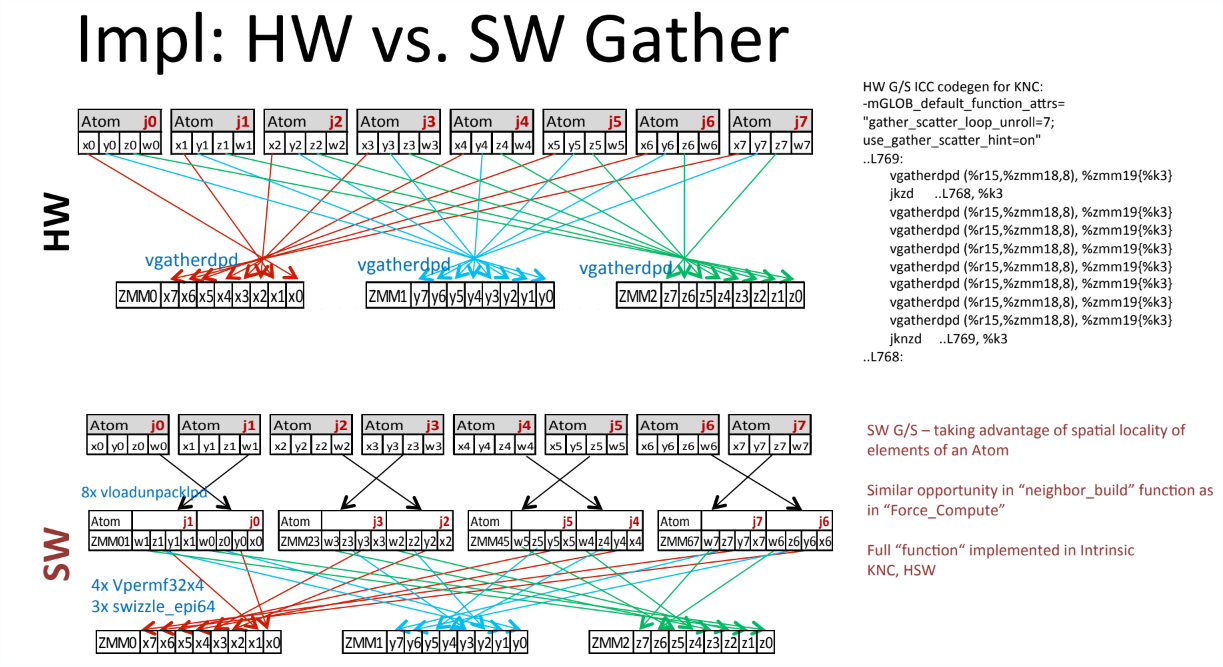
\includegraphics[width=12cm]{hw_vs_sw_gather_md.png}
  \end{frame}

  \begin{frame}[fragile]{Hardware vs. Software gather}
  \centering
    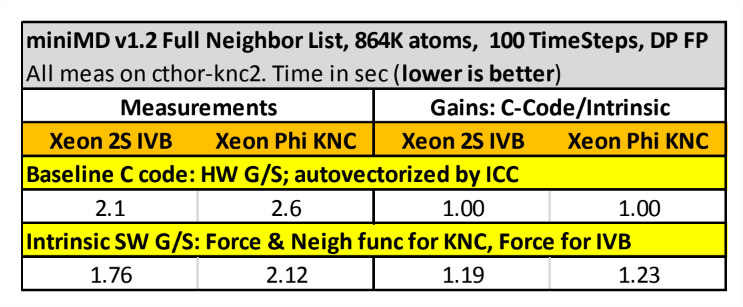
\includegraphics[width=10cm]{minimd_hw_vs_sw_results_table.png}
  \end{frame}

  \begin{frame}[fragile]{Assembly Analysis}
    \begin{itemize}
      \item Intel compiler (ICC) v19.0.5.281 Build 20190815
      \item Flags: \texttt{-S -masm=intel -D\_GNU\_SOURCE -DAOS -DPRECISION=2 -DALIGNMENT=64 -restrict -Ofast -xCORE-AVX 512 -qopt-zmm-usage=high -o ICC/force.s}
      \item For AVX512, all kernels with zmm registers and gather instructions
      \item Three kernel variants are generated by the compiler (Consider \texttt{rmng\_neighs = numneighs - k}):
      \begin{itemize}
        \item \texttt{rmng\_neighs < 8:} last iteration, vectors are not fulfilled
        \item \texttt{rmng\_neighs in ]8, 1200]:} with mov+lea instructions (prefetching?), L1 case? 1200 * 3 * 8 = 28.8kB, L1 cache size is 32kB on Cascade Lake
        \item \texttt{rmng\_neighs >= 1200:} no mov+lea instructions
      \end{itemize}
      \item We will focus on the \texttt{rmng\_neighs in ]8, 1200]} variant
    \end{itemize}
  \end{frame}

  \begin{frame}[fragile]{Assembly Analysis:}
    \begin{lstlisting}[basicstyle=\tt\tiny]
vmovdqu   ymm3, YMMWORD PTR [r13+rbx*4]         # ymm3 <- neighs[k]
vpaddd    ymm4, ymm3, ymm3                      # ymm4 <- neighs[k] * 2
vpaddd    ymm3, ymm3, ymm4                      # ymm3 <- neighs[k] * 3
# -------------------- mov+lea instructions (prefetching?) -----------------------
mov       r10d, DWORD PTR [r13+rbx*4]           # r10d <- neighs[k]
mov       r9d, DWORD PTR [4+r13+rbx*4]          # r9d  <- neighs[k + 1]
mov       r8d, DWORD PTR [8+r13+rbx*4]          # r8d  <- neighs[k + 2]
mov       esi, DWORD PTR [12+r13+rbx*4]         # esi  <- neighs[k + 3]
lea       r10d, DWORD PTR [r10+r10*2]           # r10d <- neighs[k] * 3
mov       ecx, DWORD PTR [16+r13+rbx*4]         # ecx  <- neighs[k + 4]
lea       r9d, DWORD PTR [r9+r9*2]              # r9d  <- neighs[k + 1] * 3
mov       edx, DWORD PTR [20+r13+rbx*4]         # edx  <- neighs[k + 5]
lea       r8d, DWORD PTR [r8+r8*2]              # r8d  <- neighs[k + 2] * 3
mov       eax, DWORD PTR [24+r13+rbx*4]         # edx  <- neighs[k + 6]
lea       esi, DWORD PTR [rsi+rsi*2]            # esi  <- neighs[k + 3] * 3
mov       r15d, DWORD PTR [28+r13+rbx*4]        # edx  <- neighs[k + 7]
lea       ecx, DWORD PTR [rcx+rcx*2]            # ecx  <- neighs[k + 4] * 3
lea       edx, DWORD PTR [rdx+rdx*2]            # edx  <- neighs[k + 5] * 3
lea       eax, DWORD PTR [rax+rax*2]            # eax  <- neighs[k + 6] * 3
lea       r15d, DWORD PTR [r15+r15*2]           # r15d <- neighs[k + 7] * 3
# -------------------- end of mov+lea instructions -------------------------------
vpcmpeqb  k1, xmm0, xmm0                        # k1    <- [true for all elements]
vpcmpeqb  k2, xmm0, xmm0                        # k2    <- [true for all elements]
vpcmpeqb  k3, xmm0, xmm0                        # k3    <- [true for all elements]
vpxord    zmm4, zmm4, zmm4                      # zmm4  <- 0.0
vpxord    zmm17, zmm17, zmm17                   # zmm17 <- 0.0
vpxord    zmm18, zmm18, zmm18                   # zmm18 <- 0.0
vgatherdpd zmm4{k1}, QWORD PTR [16+rdi+ymm3*8]  # zmm4  <- atom->x[j * 3 + 2]
vgatherdpd zmm17{k2}, QWORD PTR [8+rdi+ymm3*8]  # zmm17 <- atom->x[j * 3 + 1]
vgatherdpd zmm18{k3}, QWORD PTR [rdi+ymm3*8]    # zmm18 <- atom->x[j * 3]
    \end{lstlisting}
  \end{frame}

  \begin{frame}[fragile]{Assembly Analysis:}
    When removing mov+lea instructions, performance is better on Cascade Lake:
    \begin{verbatim}
    With lea+mov:
    TOTAL 9.30s FORCE 4.81s NEIGH 4.25s REST 0.24s

    Without lea+mov:
    TOTAL 8.95s FORCE 4.43s NEIGH 4.28s REST 0.24s
    \end{verbatim}
  \end{frame}

  \begin{frame}[fragile]{Stubbed Force Calculation}
    \begin{itemize}
      \item Goal: core execution time contribution
      \item Execute most internal loop with data fitting into cache sizes
      \item Keep number of neighbors per atom fixed
      \item Compare cycles per iteration with OSACA and IACA outputs
    \end{itemize}
  \end{frame}

  \begin{frame}{Stubbed Force Calculation}
  \centering
    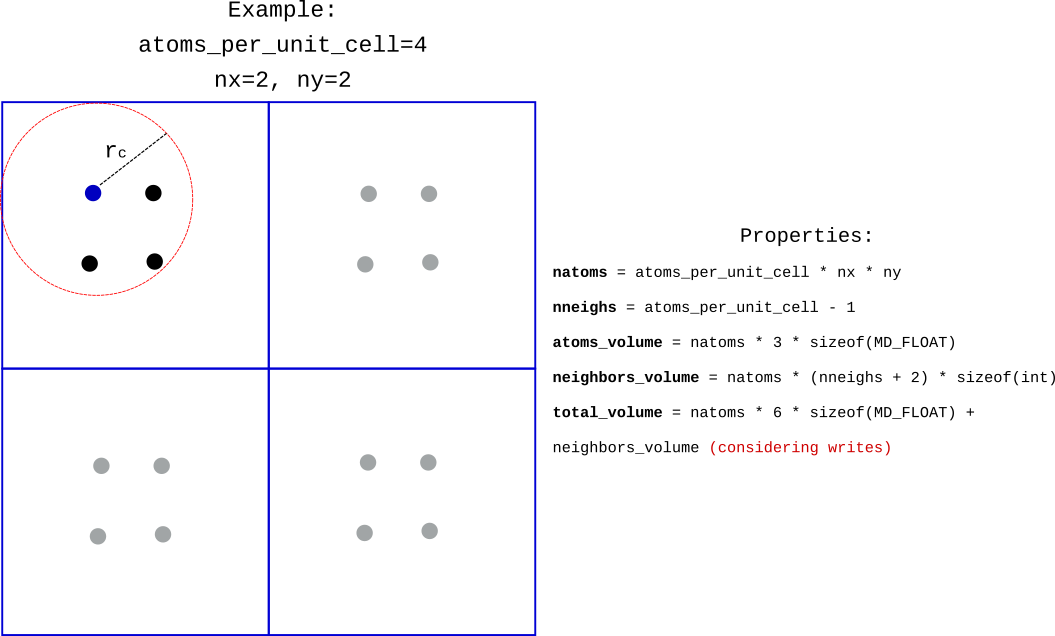
\includegraphics[width=9cm]{stubbed_force_mdbench.png}
  \end{frame}

  \begin{frame}[fragile]{OSACA Analysis}
    \begin{lstlisting}[basicstyle=\tt\tiny]
                                     Port pressure in cycles                                     
     |  0   - 0DV  |  1   |  2   -  2D  |  3   -  3D  |  4   |  5   |  6   |  7   ||  CP  | LCD  |
-------------------------------------------------------------------------------------------------
 260 |             |      | 0.50   0.50 | 0.50   0.50 |      |      |      |      ||  4.0 |      |   vmovdqu   (%rcx,%r14,4), %ymm3                          #68.21
 261 | 0.00        | 0.50 |             |             |      | 0.00 | 0.50 |      ||      |      |   addq      $8, %r14                                      #67.9
 262 | 0.50        |      |             |             |      | 0.50 |      |      ||      |      |   vpxord    %zmm5, %zmm5, %zmm5                           #70.36
 263 | 0.50        |      |             |             |      | 0.50 |      |      ||      |      |   vpxord    %zmm4, %zmm4, %zmm4                           #69.36
 264 | 0.50        |      |             |             |      | 0.50 |      |      ||      |      |   vpxord    %zmm6, %zmm6, %zmm6                           #71.36
 265 | 1.50        | 0.50 | 4.00   0.50 | 4.00   0.50 |      | 0.50 | 0.50 |      ||  4.0 |      |   vgatherdpd (%rax,%ymm3,8), %zmm5{%k2}                   #70.36
 266 | 1.50        | 0.50 | 4.00   0.50 | 4.00   0.50 |      | 0.50 | 0.50 |      ||      |      |   vgatherdpd (%rdx,%ymm3,8), %zmm4{%k1}                   #69.36
 267 | 1.50        | 0.50 | 4.00   0.50 | 4.00   0.50 |      | 0.50 | 0.50 |      ||      |      |   vgatherdpd (%rsi,%ymm3,8), %zmm6{%k3}                   #71.36
 268 | 0.50        |      |             |             |      | 0.50 |      |      ||  4.0 |      |   vsubpd    %zmm5, %zmm1, %zmm29                          #70.36
 269 | 0.50        |      |             |             |      | 0.50 |      |      ||      |      |   vsubpd    %zmm4, %zmm0, %zmm28                          #69.36
 270 | 0.50        |      |             |             |      | 0.50 |      |      ||      |      |   vsubpd    %zmm6, %zmm2, %zmm31                          #71.36
 271 | 0.50        |      |             |             |      | 0.50 |      |      ||  4.0 |      |   vmulpd    %zmm29, %zmm29, %zmm20                        #72.49
 272 | 0.50        |      |             |             |      | 0.50 |      |      ||  4.0 |      |   vfmadd231pd %zmm28, %zmm28, %zmm20                      #72.49
 273 | 0.50        |      |             |             |      | 0.50 |      |      ||  4.0 |      |   vfmadd231pd %zmm31, %zmm31, %zmm20                      #72.63
 274 | 2.50        |      |             |             |      | 0.50 |      |      ||  8.0 |      |   vrcp14pd  %zmm20, %zmm27                                #75.38
 275 |             |      |             |             |      | 1.00 |      |      ||      |      |   vcmppd    $1, %zmm16, %zmm20, %k5                       #74.22
 276 |             |      |             |             |      | 1.00 |      |      ||      |      |   vfpclasspd $30, %zmm27, %k0                             #75.38
 277 | 0.50        |      | 0.50   0.50 | 0.50   0.50 |      | 0.50 |      |      ||  4.0 |      |   vfnmadd213pd .L_2il0floatpacket.5(%rip){1to8}, %zmm27, %zmm20 #75.38
 278 | 1.00        |      |             |             |      |      |      |      ||      |      |   knotw     %k0, %k4                                      #75.38
 279 | 0.50        |      |             |             |      | 0.50 |      |      ||  4.0 |      |   vmulpd    %zmm20, %zmm20, %zmm21                        #75.38
 280 | 0.50        |      |             |             |      | 0.50 |      |      ||      |      |   vfmadd213pd %zmm27, %zmm20, %zmm27{%k4}                 #75.38
 281 | 0.50        |      |             |             |      | 0.50 |      |      ||  4.0 |      |   vfmadd213pd %zmm27, %zmm21, %zmm27{%k4}                 #75.38
 282 | 0.50        |      |             |             |      | 0.50 |      |      ||  4.0 |      |   vmulpd    %zmm15, %zmm27, %zmm22                        #76.38
 283 | 0.50        |      |             |             |      | 0.50 |      |      ||      |      |   vmulpd    %zmm14, %zmm27, %zmm24                        #77.54
 284 | 0.50        |      |             |             |      | 0.50 |      |      ||  4.0 |      |   vmulpd    %zmm22, %zmm27, %zmm25                        #76.44
 285 | 0.50        |      |             |             |      | 0.50 |      |      ||  4.0 |      |   vmulpd    %zmm25, %zmm27, %zmm23                        #76.50
 286 | 0.50        |      |             |             |      | 0.50 |      |      ||      |      |   vfmsub213pd %zmm7, %zmm25, %zmm27                       #77.54
 287 | 0.50        |      |             |             |      | 0.50 |      |      ||  4.0 |      |   vmulpd    %zmm24, %zmm23, %zmm26                        #77.61
 288 | 0.00        |      |             |             |      | 1.00 |      |      ||  4.0 |      |   vmulpd    %zmm27, %zmm26, %zmm30                        #77.67
 289 | 0.00        |      |             |             |      | 1.00 |      |      ||      |      |   vfmadd231pd %zmm28, %zmm30, %zmm13{%k5}                 #78.17
 290 | 0.00        |      |             |             |      | 1.00 |      |      ||      |  4.0 |   vfmadd231pd %zmm29, %zmm30, %zmm12{%k5}                 #79.17
 291 | 0.00        |      |             |             |      | 1.00 |      |      ||  4.0 |      |   vfmadd231pd %zmm31, %zmm30, %zmm11{%k5}                 #80.17
 292 | 0.00        | 0.50 |             |             |      | 0.00 | 0.50 |      ||      |      |   cmpl      %ebx, %r9d                                    #67.9
 293 |             |      |             |             |      |      |      |      ||      |      | * jb        ..B1.22       # Prob 82%                      #67.9

       17.5          3.00   13.0   2.50   13.0   2.50          17.5   3.00           68.0    4   


Loop-Carried Dependencies Analysis Report
-----------------------------------------
 257 |  1.0 | addl      $8, %r9d                                      #67.9| [257]
 261 |  1.0 | addq      $8, %r14                                      #67.9| [261]
 290 |  4.0 | vfmadd231pd %zmm29, %zmm30, %zmm12{%k5}                 #79.17| [290]
 289 |  4.0 | vfmadd231pd %zmm28, %zmm30, %zmm13{%k5}                 #78.17| [289]
 291 |  4.0 | vfmadd231pd %zmm31, %zmm30, %zmm11{%k5}                 #80.17| [291]
    \end{lstlisting}
  \end{frame}

  \begin{frame}[fragile]{Running Internal Loop several times}
  \end{frame}

  \begin{frame}[fragile]{Cycles when running internal loop several time}
  \end{frame}

  \begin{frame}[fragile]{Conclusions about Texec}
  \end{frame}

  \begin{frame}[fragile]{gather-bench}
  \end{frame}

  % List example
  %\begin{frame}[fragile]{Capturing expressions}
  %  \begin{itemize}
  %      \item Operator overloading
  %      \item Vector operations are easily expressed
  %  \end{itemize}
  %\end{frame}

  % Code example
  %\begin{frame}[fragile]{Capturing expressions}
  %  \begin{lstlisting}
  %  \end{lstlisting}
  %\end{frame}

  % Image example
  %\begin{frame}{Experimental Results}
  %  \begin{block}{Weak Scaling Perfomance}
  %    \includegraphics[width=9cm]{results/weak_scaling.png}
  %  \end{block}
  %\end{frame}

  { % Questions?
    %\setbeamertemplate{footline}{}
    %\begin{frame}[c,noframenumbering]
    %  \begin{center}
    %    Thank you for listening.\\
    %    {\bf Any questions?}
    %  \end{center}
    %\end{frame}

    % References
    %\section*{References}
    %\begin{frame}[allowframebreaks,noframenumbering]{References}
    %  \printbibliography
    %\end{frame}
  }
\end{document}

